\documentclass[12pt]{article}                                                                                                                       
\usepackage{sbc-template}                                                 
\usepackage{graphicx,url}                                                 
\usepackage[utf8]{inputenc}                                               
\usepackage[brazil]{babel}                                                      
\usepackage{graphicx}

\title{Trabalho Prático\\ Vinho e qualidade:\\ Uma análise utilizando Machine Learning}
\author{Iyan Lucas Duarte Marques\inst{1}, Samir do Amorim Cabraia\inst{1}, Wesley Filemon Rocha Rodrigues\inst{1}}

\address{Instituto de Ciências Exatas e Informática - Pontifícea Universidade Católica Minas Gerais (PUC-MG)}

\begin{document}

\maketitle

\section{Introdução}

\section{Base de Dados}
A base utilizada é a \textit{Wine Quality Data Set}, disponível no \textit{UCI Machine Learning Repository}.
A mesma foi introduzida em um paper por Paulo Cortez ~\cite{vinho} que propõe uma forma de predição das preferências de gosto e qualidade de vinho do homem.
Desta forma, a base consiste em análise de críticos do vinho \textit{"Vinho Verde"}\footnote{
	Companhia portuguesa de vinhos e adegas. Mais informações: https://www.vinhoverde.pt
} português.
Há duas tabelas, uma de vinho branco com 4898 instâncias e de vinho tinto com 1599 instâncias, para a finalidade deste trabalho, se utilizou somente a base de vinhos brancos, pela quantidade e estado das instâncias.
Eles são classificados de um score de 0 a 10, sendo 0 muito ruim e 10 extremamente excelente. 
Este score (atributo 12) é o resultado entre a média dos resultados dados por 3 sommeliers experts. 

\subsection{Atribustos}
São 12 atributos, cada um representando um teste objetivo:
\begin{itemize}
	\item 1 - Acides fixa
	\item 2 - Acides volátil
	\item 3 - Acido cítrico
	\item 4 - Açúcar residual
	\item 5 - Clorídeos
	\item 6 - Dióxido de enxofre livre
	\item 7 - Total de dióxido de enxofre
	\item 8 - Densidade
	\item 9 - pH
	\item 10 - Sulfatos
	\item 11 - álcool
	\item 12 - qualidade (score entre 0 e 10)
\end{itemize}


\section{Resultados Preliminares}

% Several data mining methods were applied to model
% these datasets under a regression approach. The support vector machine model achieved the
% best results. Several metrics were computed: MAD, confusion matrix for a fixed error tolerance (T),
% etc. Also, we plot the relative importances of the input variables (as measured by a sensitivity
% analysis procedure).

Ao acessar e estudar a base, percebe-se que a mesma está relativamente desbalanceada. 
Há mais vinhos normais do que ruins ou excelentes, apesar de que as classes estão ordenadas.
Desta forma, para medida de comparação, foi executado na plataforma WEKA\footnote{
	Waikato Environment for Knowledge Analysis
} o algoritmo Random Forest, o qual apresentou os seguintes resultados: 

\begin{figure}[h]
	\begin{small}
		\begin{center}
			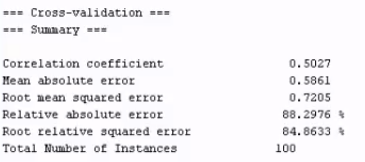
\includegraphics[]{figures/1.png}
		\end{center}
		\caption{Resultados com a base desbalanceada}
		\label{fig:unballanced}
	\end{small}
\end{figure}



Analisando os resultados, é evidente que a base está com algum conflito, decorrências do desbalanceamento. 
Conforme o resultado, o time se empenhou em atingir um método de que se faça o balanceamento de forma que se mantenha a integridade da base e o numero médio de instâncias.
Após reuniões, concluimos que o algoritmo que apresentou os melhores resultados foi o Resample\footnote{
	Produz uma subamostra aleatória de um conjunto de dados usando amostragem com substituição ou sem substituição.
}, que apresentou os seguintes resultados a partir do Random Forest

\begin{figure}[h]
	\begin{small}
		\begin{center}
			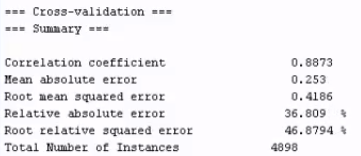
\includegraphics[]{figures/2.png}
		\end{center}
		\caption{Resultados com a base desbalanceada}
		\label{fig:ballanced}
	\end{small}
\end{figure}

Analisando os resultados do balanceamento, é perceptível uma melhora de mais de 50\% em todos os atributos gerados pelo \textit{output} do método.




\bibliography{base-referencias}
\bibliographystyle{ieeetr}
\end{document}
